\documentclass[13pt]{beamer}
\usetheme[sectionpage=progressbar,numbering=fraction,progressbar=frametitle]{metropolis}
%\usecolortheme{dove}
\usepackage{etoolbox}
\usepackage{ragged2e}
\usepackage[utf8]{inputenc}
\usepackage[italian]{babel}
\usepackage{scrextend}
%\usepackage{tikz}
%\usepackage{adjustbox}
%\usepackage{multirow}
%\usepackage{media9}
\usepackage{pgf}  

%\AtBeginSection[]{\frame{\Large \centering \insertsection} \subsection{} }
%\AtBeginSection[]{\subsection{}}

\newcommand{\nologo}{\setbeamertemplate{logo}{}}

\apptocmd{\frame}{}{\justifying}{}

\author{Cap. Alberto Azzalini}
\title[Legalità]{Introduzione alla legalità}
%\subtitle{Introduzione alle modalità operative}

\setbeamercolor{section}{ bg=black}

\logo{
\includegraphics[width=1cm]{pics/logo.png}}


\institute{
\includegraphics[width=2cm]{pics/logo.png} \\ A cura della Compagnia Carabinieri di Vipiteno}

%\date{8 aprile 2016}

%subject{}

\setbeamercovered{transparent}

%\setbeamertemplate{navigation symbols}{}

\begin{document}
	{
	\nologo
	\maketitle
	}
	\begin{frame}
		\frametitle{Indice dei contenuti}
		\tableofcontents
	\end{frame}

	\section[Compiti di polizia]{I Carabinieri e i compiti di polizia}
	\begin{frame}
		\frametitle{I principali compiti di polizia}
		\framesubtitle{Cosa fanno i Carabinieri?}
		
		\vfill
		\begin{itemize}
			\item Polizia di sicurezza:

			\begin{itemize}
				\item pronto intervento (112);
				\item prevenzione dei reati;
			\end{itemize}
			\vfill
			\item Polizia Giudiziaria:

			\begin{itemize}
				\item indagini;
				\item repressione dei reati;
			\end{itemize}
		\end{itemize}
	\end{frame}
	
	\begin{frame}
		\frametitle{La ``legalità''}
		\'{E} l'insieme delle regole, scritte e non, grazie alle quali la nostra società può funzionare, garantendo che tutti possa godere dei diritti fondamentali.
		\vfill
		In un mondo perfetto, basterebbero le regole dettate dal buon senso, ma nel mondo reale abbiamo bisogno delle \textbf{leggi}.
		
	\end{frame}
	
	\begin{frame}
		\frametitle{Il concetto di reato (1/2)}
		Il reato è un comportamento per il quale la legge prevede una pena detentiva (reclusione o arresto) e/o una pena pecuniaria (multa o ammenda).
	\end{frame}
	
	\begin{frame}
		\frametitle{Il concetto di reato (2/2)}
		
			\setbeamercovered{invisible}
			\onslide<1->{Come sono formulati i reati?}
			\setbeamercovered{invisible}
			\onslide<2>{
				
			Nell'ordinamento italiano la legge raramente pone esplicitamente dei divieti: di solito indica la pena a cui soggiace chi mette in atto un comportamento lesivo di un bene giuridico tutelato.}
	\end{frame}
	
	\begin{frame}
		\frametitle{L'imputabilità}
%		È la ``idoneità al reato'', ovvero la condizione sufficiente ad attribuire a un soggetto l'azione penale e a mettere in conto le conseguenze giuridiche.
		È la condizione necessaria perché una persona possa essere chiamata a rispondere penalmente di un fatto commesso.
		\vfill
		È ``imputabile'' chi:
		\begin{itemize}
			\item ha compiuto 14 anni;
			\item è capace di \underline{intendere} e di \underline{volere}.
		\end{itemize}
		
	\end{frame}

	\begin{frame}
		\frametitle{Intendere e volere}
		\textbf{Capacità di intendere}\\
		comprendere il significato delle proprie azioni e accettarne consapevolmente le conseguenze.
		\vfill
		\textbf{Capacità di volere} \\
		avere il controllo dei propri stimoli e impulsi ad agire e volontariamente mettere in atto le azioni compiute.
	\end{frame}	

	\begin{frame}
		\frametitle{La responsabilità}
			\textbf{Responsabilità penale}\\ ciascuno risponde personalmente delle proprie azioni e nessuno va in carcere per reati commessi da altre persone.
			\vfill
			\textbf{Responsabilità civile}\\ i genitori non vanno in carcere per i reati commessi dai loro figli, ma possono essere costretti a risarcire i danni che hanno commesso.
	\end{frame}	
	
	\begin{frame}
		\frametitle{Dei semplici esempi}
		\begin{columns}[T]
			\begin{column}{.5\textwidth}
				\begin{block}{}
					Due piccoli criminali \\
%				\end{block}
%				\begin{block}{}	
					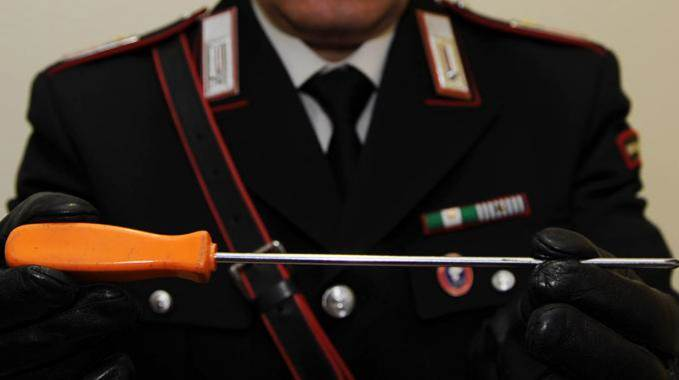
\includegraphics[width=\textwidth]{pics/cacciavite.jpg}
				\end{block}
			\end{column}
			\begin{column}{.5\textwidth}
				\begin{block}{}
					% Your image included here
					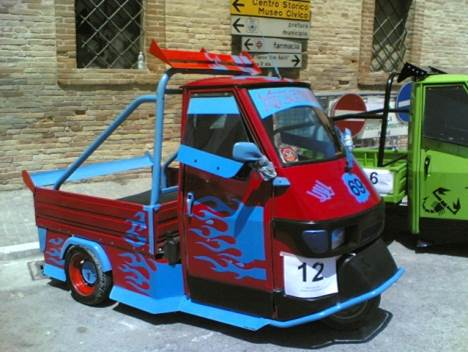
\includegraphics[width=\textwidth]{pics/ape.jpg}
%				\end{block}
%				\begin{block}{}
					\\ e un'Ape truccata.
				\end{block}
			\end{column}
		\end{columns}
	\end{frame}
	
	\section[Bullismo]{Il Bullismo - Conoscerlo e prevenirlo}

	\begin{frame}
		\frametitle{Definizione di bullismo (1/2)}
		Il termine bullismo deriva dalla parola inglese ``bullying'' e viene definito come un'oppressione, psicologica o fisica, ripetuta e continuata nel tempo, perpetrata da una persona  o da un gruppo di persone più potente nei confronti di un'altra percepita come più debole.
	\end{frame}
	\begin{frame}
		\frametitle{Definizione di bullismo (2/2)}
		Una definizione sociologica:
		
		\begin{quote}
			Un comportamento bullo è un tipo di azione che mira \textbf{deliberatamente} a far del male o a danneggiare; spesso è \textbf{persistente}, talvolta dura per settimane, mesi, persino anni ed è \textbf{difficile difendersi} per coloro che ne sono vittime. Alla base della maggior parte dei comportamenti sopraffattori c'è un \textbf{abuso di potere} e un desiderio di \textbf{intimidire e dominare}.
			\hfill (Sharp e Smith, 1995)
		\end{quote}		
	\end{frame}

	\begin{frame}
		\frametitle{Caratteristiche del bullismo}
		
		\begin{itemize}
			\item intenzionalità;
			\item durata nel tempo;
			\item disuguaglianza tra bullo e vittima;
			\item mancanza di sostegno per la vittima;
			\item danno per l'autostima della vittima;
			
		\end{itemize}
		
	\end{frame}

	\begin{frame}
		\frametitle{Le forme del bullismo}
		\begin{description}
			\item[fisico]
			\begin{itemize}
				\item aggressioni fisiche;
				\item furti;
				\item danneggiamenti;
			\end{itemize}
			\item[verbale]
			\begin{itemize}
				\item minacce;
				\item insulti e offese anche razziste;
				\item estornsioni;
			\end{itemize}
			\item[indiretto]
			\begin{itemize}
				\item diffusione di pettegolezzi e calunnie;
				\item esclusione dal gruppo e isolamento;
				\item danneggiamento dei rapporti di amicizia.
			\end{itemize}
		\end{description}
	\end{frame}

	\begin{frame}
		\frametitle{Il bullismo è maschio o femmina?}
		In generale valgono queste ``regole'':
		\begin{itemize}
			\item il bullismo riguarda sia maschi che femmine;
			\item i maschi di solito attaccano indifferentemente maschi o femmine;
			\item le femmine tendono a mettere in atto prepotenze indirette (psicologiche) quasi sempre nei confronti di altre ragazze.
		\end{itemize}
	\end{frame}

	\begin{frame}
		\frametitle{I tempi e i luoghi del bullismo}
		Gli episodi di bullismo di verificano generalmente:
		\begin{itemize}
			\item tra i 7 e i 16 anni;
			\item all'interno della scuola lontano dalla vista degli insegnanti;
			\item nel tragitto casa-scuola e negli altri luoghi di ritrovo.
		\end{itemize}
		Il bullo cerca e sceglie la sua vittima a scuola, ma mette in atto i suoi comportamenti solo dove gli spettatori possono essere dalla sua parte.
	\end{frame}
	
	\begin{frame}
		\frametitle{Non tutto è bullismo}
		Atteggiamenti ``quasi aggressivi'' quali:
		
		\begin{itemize}
			\item giochi turbolenti;
			\item occasionali litigi;
			\item zuffe per futili motivi;
			\item scherzose prese in giro,
		\end{itemize}
		\alert{non sempre sono bullismo}: per esserlo, devono avere le caratteristiche già richiamate (\textbf{intenzionalità}, \textbf{durata}, \textbf{asimmetria},\dots)
		
		\textit{Tuttavia sono comunque comportamenti esecrabili, che possono e devono essere puniti dagli insegnanti!}
	\end{frame}	

	\begin{frame}
		\frametitle{Oltre il bullismo}
		Quando il bullismo diventa:
		\begin{itemize}
			\item minacce;
			\item furti;
			\item molestie e abusi sessuali;
			\item lesioni personali;
			\item razzismo;
			\item offese, calunnie e voci diffamatorie,
		\end{itemize}
	siamo ormai nell'ambito di veri e propri \alert{reati} che come tali devono essere perseguiti.
	\end{frame}

	\begin{frame}
		\frametitle{Luoghi comuni errati e false convinzioni}
		\textbf{Non è vero} che il bullismo\dots
		\begin{itemize}
			\item in fondo è solo ``una ragazzata'';
			\item fa parte della crescita;
			\item è un fenomeno proprio delle zone più povere e degradate;
			\item deriva dalla competizione per ottenere buoni voti a scuola.
		\end{itemize}
		
		\textbf{Chi subisce prepotenze dai bulli non può divendersi da solo!}
		
	\end{frame}

	\begin{frame}
		\frametitle{L'importanza del gruppo}
		Chi assiste a episodi di bullismo, con il proprio comportamento, può favorire o frenare le azioni del bullo.
		
		Ciascuno ha l'obbligo morale di difendere le vittime dei bulli:
		\begin{itemize}
			\item direttamente, intervenendo se se la sente;
			\item chiedendo aiuto agli adulti;
			\item \textbf{denunciando i bulli}.
		\end{itemize}
		
		Ammirare le azioni del bullo significa:
		\begin{itemize}
			\item \textbf{ammirare un vigliacco};
			\item invogliarlo a continuare con le sue pessime azioni.
		\end{itemize} 
	\end{frame}

	\begin{frame}
		\frametitle{Come contrastare il fenomeno (1/2)}
		\textbf{Strategie attive}:
		\begin{itemize}
			\item richiedere l'aiuto di un adulto;
			\item esprimere apertamente a livello verbale la disapprovazione per i comportamenti prevaricatori, dicendo esplicitamente al bullo di smetterla;
			\item cercare di aiutare la vittima a sottrarsi alla situazione;
			\item sollecitare i compagni a non appoggiare i bulli.
		\end{itemize}
	\end{frame}

	\begin{frame}
		\frametitle{Come contrastare il fenomeno (2/2)}
		\textbf{Strategie passive}:
		\begin{itemize}
			\item rifiutare di prendere parte alla situazione;
			\item esprimere a livello non verbale il rifiuto di prendere parte alle prepotenze;
			\item aprire il proprio gruppo alla vittima.
			
		\end{itemize}
	\end{frame}

	\begin{frame}
		\frametitle{Trovare aiuto}	
		Del bullismo si deve parlare e va denunciato!
		
		A chi rivolgersi:
		\begin{itemize}
			\item genitori;
			\item insegnanti;
			\item forze dell'ordine;
			\item servizi sociali.
		\end{itemize}
	\end{frame}
	
	\begin{frame}[standout]
		Nessuno merita di subire prepotenze, \\ ma da soli non si sconfigge il bullismo:


		\alert{contro il bullismo, l'unione fa la forza!}
		
	\end{frame}

%	\begin{frame}
%		\frametitle{}
%		
%	\end{frame}

	\section{Internet e i rischi connessi}
	\begin{frame}
		\frametitle{Le componenti del rischio}
		Distinguiamo quattro pericoli legati alle attività \textit{on-line}:
		\begin{itemize}
			\onslide<2->\item rischio per l'incolumità fisica;
			\onslide<3->\item rischio per l'immagine;
			\onslide<4->\item rischio di essere vittima di reati;
			\onslide<5>\item rischio di commettere reati.
		\end{itemize}
	\end{frame}

	\begin{frame}[standout]
		Una regola d'oro:
	
		\alert{Se una cosa non la farei nel mondo reale,\\
		probabilmente non è il caso di farla \textit{on-line}}
		
	\end{frame}

	\begin{frame}
		\frametitle{L'incolumità fisica}
		Le tecniche dell'adescamento \textit{on-line} di giovani vittime:
		\begin{itemize}
			\item {guadagnare fiducia;}
			\item {creare empatia;}
			\item {abbassare le difese;}
			\item {mettere a proprio agio;}
			\item {ingegneria sociale.}
		\end{itemize}
		Su Internet si tende ad essere meno diffidenti e a dare fiducia a chiunque.
	\end{frame}

	\begin{frame}
		\frametitle{Come difendersi}
		Su Internet, nelle chat, nei giochi di ruolo:
		\begin{itemize}
			\item non dare MAI informazioni personali;
			\item non inviare foto intime e non accettarne;
			\item non incontrare MAI persone conosciute solo \textit{on-line};
			\item se ti senti a disagio, smetti di chattare, cambia indirizzo email e \alert{avvisa i tuoi genitori};
			\item diffida sempre di chi ti sembra troppo simpatico.
		\end{itemize}
		Ricorda che lo schermo nasconde le vere intenzioni del tuo interlocutore: dietro al computer è molto facile fingere.
	\end{frame}

	\begin{frame}[standout]

		\onslide<1->{Cosa significa \\ ``Non accettare caramelle dagli sconosciuti''?}
		
		\setbeamercovered{invisible}
		\onslide<2>{\alert{Significa non fidarsi mai di chi non si conosce.}}
		
	\end{frame}



%	\begin{frame}
%		\frametitle{}
%		
%	\end{frame}

%	\begin{frame}
%		\frametitle{}
%		
%	\end{frame}

%	\begin{frame}
%		\frametitle{}
%		
%	\end{frame}

%	\begin{frame}
%		\frametitle{}
%		
%	\end{frame}

%	\begin{frame}
%		\frametitle{}
%		
%	\end{frame}

%	\begin{frame}
%		\frametitle{}
%		
%	\end{frame}

%	\begin{frame}
%		\frametitle{}
%		
%	\end{frame}

%	\begin{frame}
%		\frametitle{}
%		
%	\end{frame}

%	\begin{frame}
%		\frametitle{}
%		
%	\end{frame}

%	\begin{frame}
%		\frametitle{}
%		
%	\end{frame}

%	\begin{frame}
%		\frametitle{}
%		
%	\end{frame}

%	\begin{frame}
%		\frametitle{}
%		
%	\end{frame}

%	\begin{frame}
%		\frametitle{}
%		
%	\end{frame}

%	\begin{frame}
%		\frametitle{}
%		
%	\end{frame}

%	\begin{frame}
%		\frametitle{}
%		
%	\end{frame}

%	\begin{frame}
%		\frametitle{}
%		
%	\end{frame}

%	\begin{frame}
%		\frametitle{}
%		
%	\end{frame}

%	\begin{frame}
%		\frametitle{}
%		
%	\end{frame}

%	\begin{frame}
%		\frametitle{}
%		
%	\end{frame}

	
%	\begin{frame}
%		\begin{center}%
%			\includemedia[
%			width=10cm,
%			activate=pageopen,
%			addresource=pics/flv.flv,
%			playbutton= fancy,
%			flashvars={source=flv.flv}
%			]{Movie}{VPlayer.swf}
%		\end{center}%
%	\end{frame}
\end{document}